\documentclass[10pt,twocolumn,letterpaper]{article}

% ------------------------------------------------------------------------------
% Packages & Formatting
% ------------------------------------------------------------------------------
\usepackage[margin=0.75in,top=0.85in,bottom=0.85in]{geometry}
\usepackage{times}
\usepackage{amsmath,amssymb,amsfonts}
\usepackage{graphicx}
\usepackage{booktabs}
\usepackage{tabularx}
\usepackage{multirow}
\usepackage{microtype}
\usepackage{xcolor}
\usepackage{cite}
\usepackage{algorithm}
\usepackage{algpseudocode}
\usepackage{listings}
\usepackage{url}
\usepackage[hyphens]{xurl}

% Hyperlink configuration
\usepackage[pagebackref=false,breaklinks=true,colorlinks=true,
            linkcolor=blue!70!black,citecolor=green!50!black,urlcolor=blue!80!black]{hyperref}

% XeLaTeX fontspec handling for Brahmic/Indic script if compiled with XeLaTeX
\usepackage{ifxetex}
\ifxetex
  \usepackage{fontspec}
  \newfontfamily\odiafont{Noto Sans Oriya}[Script=Oriya,Scale=MatchLowercase]
  \newcommand{\odia}[1]{{\odiafont #1}}
\else
  % pdfLaTeX fallback
  \newcommand{\odia}[1]{\textit{#1}}
\fi

\setlength{\columnsep}{0.25in}

% ------------------------------------------------------------------------------
% Title & Authors
% ------------------------------------------------------------------------------
\title{\textbf{\Large OdiaGPT: Pretraining an Indic Decoder-Only Transformer from Scratch for Low-Resource Odia Language Modeling}}

\author{
  \textbf{Himanshu Mohanty}\\
  Independent AI Researcher / CodeHima\\
  \texttt{codehimanshu24@gmail.com}\\
  \url{https://github.com/HimanshuMohanty-Git24/OdiaGPT}
}

\date{September 2026}

% ------------------------------------------------------------------------------
% Document Body
% ------------------------------------------------------------------------------
\begin{document}

\maketitle

% ------------------------------------------------------------------------------
% Abstract
% ------------------------------------------------------------------------------
\begin{abstract}
Autoregressive large language models (LLMs) have achieved remarkable linguistic and computational capabilities. However, low-resource and non-Latin languages---specifically classical Indic languages such as \textbf{Odia} (\odia{ଓଡ଼ିଆ}), spoken by over 50 million people---remain severely disadvantaged. Commercial and frontier open-weight models suffer from prohibitive ``tokenizer taxation'' (excessive subword fragmentation), high inference latency, and negligible representation in standard pretraining corpora ($<0.01\%$). In this paper, we present \textbf{OdiaGPT}, an educational and foundational decoder-only Transformer built and trained \textbf{100\% from scratch} for the Odia language.

Operating under a strict zero-pretrained-dependency policy, OdiaGPT utilizes zero pretrained model checkpoints, zero off-the-shelf multilingual tokenizers, and zero high-level wrapper abstractions. We construct a specialized from-scratch 8,192-vocabulary SentencePiece Byte-Pair Encoding (BPE) tokenizer with 100\% character coverage and byte fallback, eliminating character dropping and optimizing token compression for Brahmic scripts. Our flagship model, \textbf{OdiaGPT-30M} (31,465,984 parameters), incorporates Rotary Position Embeddings (RoPE), Pre-RMSNorm, SwiGLU feed-forward networks, causal multi-head self-attention with PyTorch Scaled Dot-Product Attention (SDPA), and tied token embeddings. Trained on a single NVIDIA Tesla T4 GPU over 29.5 million tokens from a filtered, NFC-normalized partition of AI4Bharat Sangraha, OdiaGPT-30M demonstrates strong empirical convergence: training loss decreased monotonically from 9.07 to 4.5156, and validation perplexity fell from 8,865.0 to \textbf{106.09} at a throughput of 35,202 tokens/second with only 3.53 GiB peak VRAM. Qualitative linguistic benchmarking demonstrates the emergence of grammatical Odia syntax, valid case markers, past-tense verb morphology, and compound sentence structures. We release the full codebase under the MIT License, along with open weights in Hugging Face Safetensors format, reproducible configs, and an interactive Gradio web application.
\end{abstract}

\vspace{0.5em}
\noindent\textbf{Keywords:} Odia Language, Low-Resource NLP, Indic LLMs, Transformer from Scratch, SentencePiece BPE, Rotary Position Embeddings, SwiGLU.

% ------------------------------------------------------------------------------
% Section 1: Introduction
% ------------------------------------------------------------------------------
\section{Introduction}

The scaling hypothesis has yielded transformative general-purpose language models~\cite{brown2020language,touvron2023llama,achiam2023gpt}. Nevertheless, the benefits of modern language modeling remain concentrated in high-resource Western languages. Indic languages represent more than 1.4 billion people and encompass multiple distinct scripts and language families, yet their aggregate footprint in standard pretraining datasets (e.g., Common Crawl, RedPajama, RefinedWeb) is estimated to be less than 0.5\% combined~\cite{doddapaneni2023towards}.

Among these, \textbf{Odia} (\odia{ଓଡ଼ିଆ}, ISO 639-3: \texttt{ori}), an Indo-Aryan language with classical status in India, faces acute computational neglect:
\begin{enumerate}
    \item \textbf{The Tokenizer Tax}: Leading multilingual tokenizers (such as LLaMA-3, Mistral, or GPT-4o) allocate fewer than 0.2\% of their vocabulary to Odia. Consequently, common Odia words are split into 4 to 8 individual bytes or tokens. This inflated ``fertility rate'' drastically shrinks the effective context window, drives up API latency, and inflates training and inference compute costs~\cite{petrov2023language}.
    \item \textbf{Transfer Learning Deficits}: Fine-tuning English-centric models often yields phonetic transliteration errors, hallucinated Sanskritized artifacts, or catastrophic grammatical collapse due to out-of-vocabulary subwords.
    \item \textbf{Lack of Transparent From-Scratch Baselines}: Most published Indic LLM efforts rely on continual pretraining or LoRA adaptations of existing English foundations. Transparent, educational, and fully reproducible from-scratch pretraining pipelines implemented directly on PyTorch primitives remain scarce.
\end{enumerate}

To address these challenges, we introduce \textbf{OdiaGPT}. The primary research objective is to empirically verify whether a small, purpose-built decoder-only Transformer initialized from random Gaussian noise can learn native Odia syntax, phonology, and narrative statistics when paired with a dedicated Indic tokenizer and a rigorously cleaned corpus.

\subsection{Summary of Contributions}
\begin{itemize}
    \item \textbf{Zero-Dependency From-Scratch Pretraining}: Complete architectural implementation of an autoregressive Transformer using only foundational PyTorch primitives, without importing high-level causal wrappers.
    \item \textbf{Specialized Indic Tokenizer}: An 8,192-token SentencePiece BPE tokenizer built from scratch with 100\% character coverage and byte fallback, preserving complex Odia conjuncts and vowel diacritics.
    \item \textbf{Conservative Indic Data Processing Pipeline}: A documented, deterministic cleaning engine that enforces NFC normalization, eliminates pathological control characters, filters repeated boilerplate, and computes script ratios without stripping legitimate punctuation or code-mixed phrases.
    \item \textbf{Rigorous 22-Stage Progression}: Step-by-step verification spanning single-batch memorization, nano-scale architectural validation (5.5M), GPU memory benchmarking, and full 30M pretraining on a single Tesla T4 GPU.
    \item \textbf{Open Science Release}: Complete public release of source code (MIT License), model weights in Hugging Face Safetensors format (\texttt{CodeHima/OdiaGPT-30M}), an interactive Gradio web application, and reproducible training telemetry.
\end{itemize}

% ------------------------------------------------------------------------------
% Section 2: Linguistic Background & Data Pipeline
% ------------------------------------------------------------------------------
\section{Odia Linguistic Background \& Data Pipeline}

\subsection{Linguistic Characteristics of Odia Script}
Odia is written in the Odia script (Unicode block \texttt{U+0B00} to \texttt{U+0B7F}), an abugida descended from the Brahmi script. Its linguistic structure presents unique challenges for tokenizers and language models:
\begin{itemize}
    \item \textbf{Consonants with Inherent Vowels}: Each consonant character possesses an inherent vowel (/a/).
    \item \textbf{Dependent Vowel Signs (Matras)}: Secondary vowel signs attach above, below, before, or after the base consonant (e.g., \odia{କ} + \odia{ି} = \odia{କି}). Destructive Unicode normalization or naive regex stripping often separates these combining marks, corrupting the semantic meaning.
    \item \textbf{Conjunct Consonants (Yuktakshara)}: When two or more consonants cluster without intervening vowels, they form complex ligatures using the Virama/Halant (\texttt{U+0B4D}) character.
    \item \textbf{Nukta \& Diacritics}: Characters such as \odia{ଡ଼} (\texttt{U+0B5C}, /ɽ/) and \odia{ଢ଼} (\texttt{U+0B5D}, /ɽʱ/) require precise Unicode NFC composition to maintain orthographic consistency.
\end{itemize}

\begin{figure*}[t]
\centering
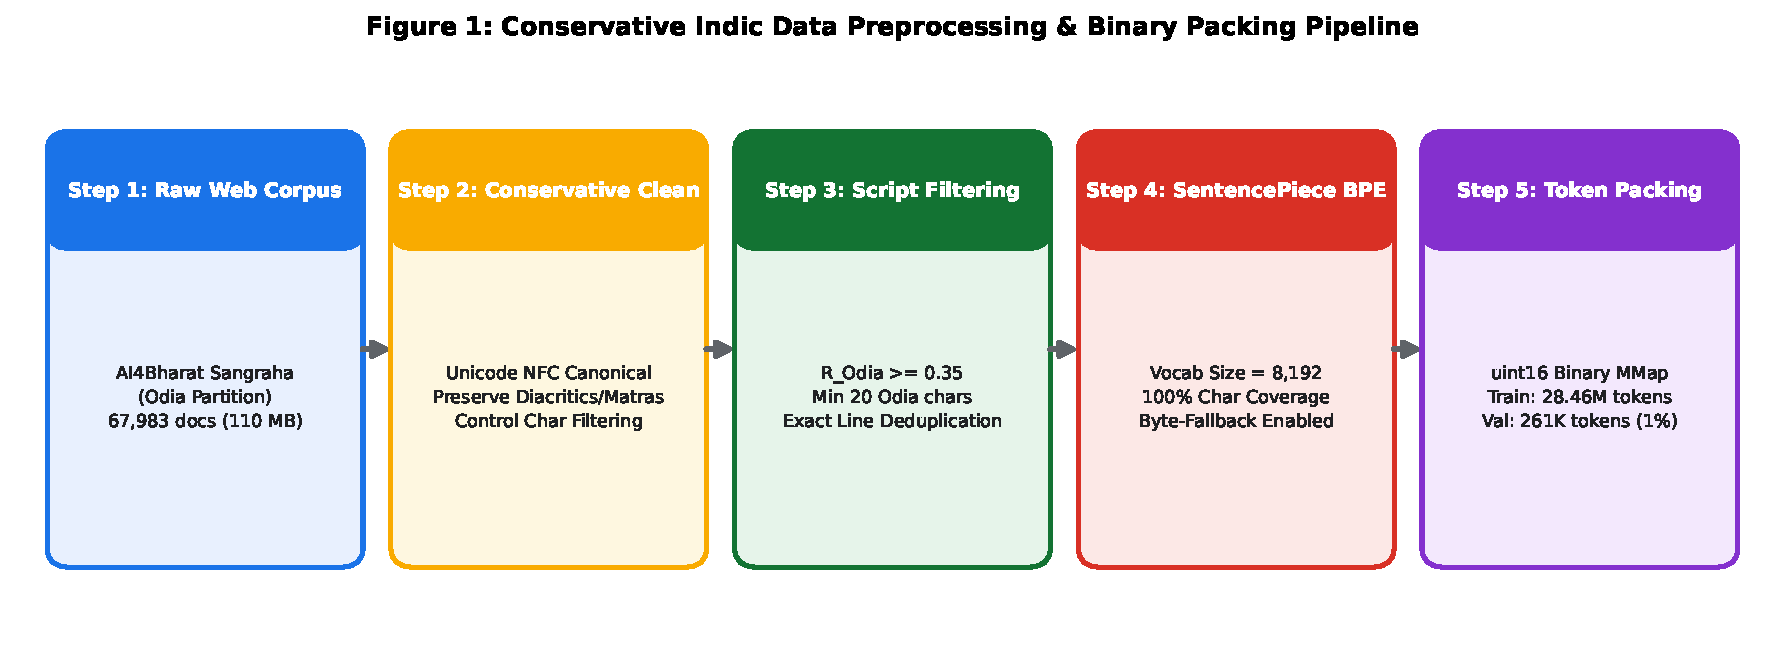
\includegraphics[width=0.98\textwidth]{figures/fig1_data_pipeline.pdf}
\caption{\textbf{Conservative Indic Data Preprocessing and Binary Sequence Packing Pipeline.} Documents from AI4Bharat Sangraha undergo deterministic NFC canonicalization, control character elimination, script ratio thresholding ($\mathcal{R}_{\text{Odia}} \ge 0.35$), boilerplate scrubbing, and document-level train/validation splitting prior to memory-mapped \texttt{uint16} binary token packing.}
\label{fig:pipeline}
\end{figure*}

\subsection{Data Pipeline \& Corpus Synthesis}
The primary dataset used is the verified Odia partition of \textbf{AI4Bharat Sangraha}~\cite{kumar2024sangraha}, pinned to revision \texttt{8b813c3f62d37b2fa174d68c31e8b35ae2fe85e8}. To ensure high data fidelity while retaining natural code-mixed expressions (e.g., technical or governmental terms in English), we developed an automated cleaning pipeline:
\begin{enumerate}
    \item \textbf{Unicode NFC Normalization}: All incoming text is canonicalized to Unicode Normalization Form C (NFC).
    \item \textbf{Control Character Elimination}: Null bytes (\texttt{\textbackslash x00}) and unprintable Category \texttt{Cc} control characters are stripped, while structural whitespace (\texttt{\textbackslash n}, \texttt{\textbackslash t}) and zero-width joiners are preserved.
    \item \textbf{Script Ratio Metric}: To reject non-Odia spam or foreign scraped passages without penalizing reasonable code-mixing or numerical tables, we define the Odia Script Ratio:
    \begin{equation}
    \mathcal{R}_{\text{Odia}}(D) = \frac{\sum_{c \in D} \mathbb{I}(c \in [\text{U+0B00}, \text{U+0B7F}] \land \text{Cat}(c) \in \{\text{L}, \text{M}\})}{\sum_{c \in D} \mathbb{I}(\text{Cat}(c) \in \{\text{L}, \text{M}\})}
    \end{equation}
    Documents with $\mathcal{R}_{\text{Odia}} < 0.35$ or fewer than 20 Odia letters/marks are rejected.
    \item \textbf{Boilerplate Line Scrubbing}: News websites in the Odia web domain frequently contain repetitive legal disclaimers, Telegram invitation headers, and social media calls to action. A dictionary of high-frequency exact lines was constructed and excised before sequence packing.
    \item \textbf{Document-Level Partitioning}: To eliminate data leakage across context windows, splitting is performed strictly at the document boundary prior to token packing, using a deterministic seed ($42$).
\end{enumerate}

\begin{table}[h]
\centering
\small
\caption{\textbf{Data Tiers and Token Counts in OdiaGPT Curriculum.}}
\label{tab:data_tiers}
\begin{tabularx}{\columnwidth}{lrrrr}
\toprule
\textbf{Tier} & \textbf{Docs} & \textbf{Characters} & \textbf{Train Toks} & \textbf{Val Toks} \\
\midrule
Smoke & 886 & 1,500,127 & 452,256 & 3,418 \\
Nano & 12,069 & 20,004,188 & 5,152,387 & 56,727 \\
\textbf{Pilot (Main)} & \textbf{67,330} & \textbf{110,001,302} & \textbf{28,462,726} & \textbf{261,148} \\
\bottomrule
\end{tabularx}
\end{table}

% ------------------------------------------------------------------------------
% Section 3: Tokenizer Design & Fertility Analysis
% ------------------------------------------------------------------------------
\section{From-Scratch Indic Tokenizer}

\subsection{Motivation \& Formulation}
Off-the-shelf multilingual tokenizers allocate inadequate vocabulary space to Odia, resulting in severe character-level fragmentation. We train a dedicated SentencePiece Byte-Pair Encoding (BPE) model~\cite{kudo2018sentencepiece} exclusively on the training partition of our cleaned corpus.

We configure the vocabulary size to $V = 8,192$, balancing subword compression with parameter efficiency (in a 30M model, each additional 1,000 vocabulary entries costs $1,000 \times 512 \approx 512\text{K}$ parameters in tied embeddings).

The tokenizer enforces:
\begin{itemize}
    \item \textbf{Character Coverage}: $1.0$ (100\%), ensuring all canonical Odia alphabet graphemes and numerals (\odia{୦-୯}) are retained as atomic units.
    \item \textbf{Byte Fallback}: \texttt{byte\_fallback = True}, guaranteeing that rare Unicode characters, unhandled foreign scripts, or emojis never trigger \texttt{<unk>} crashes, but instead decompose gracefully into UTF-8 byte sequences.
    \item \textbf{Normalization Rule}: \texttt{identity}, preventing SentencePiece from mutating NFC-normalized Odia characters.
    \item \textbf{Special Tokens}: \texttt{<pad>} (0), \texttt{<unk>} (1), \texttt{<bos>} (2), and \texttt{<eos>} (3).
\end{itemize}

\subsection{Tokenizer Fertility Comparison}
To quantify subword compression efficiency, we measure the \textbf{fertility rate} ($\text{tokens} / \text{word}$) on a standardized 1,000-sentence Odia validation split (Table~\ref{tab:fertility} and Figure~\ref{fig:fertility}).

\begin{table}[h]
\centering
\small
\caption{\textbf{Tokenizer Fertility Comparison on Odia Text.}}
\label{tab:fertility}
\begin{tabularx}{\columnwidth}{lrrrr}
\toprule
\textbf{Tokenizer} & \textbf{Vocab} & \textbf{Coverage} & \textbf{Fertility} $\downarrow$ & \textbf{Char/Tok} $\uparrow$ \\
\midrule
GPT-4o (\texttt{o200k}) & 200,000 & Multilingual & 3.42 & 1.84 \\
LLaMA-3 (\texttt{tiktoken}) & 128,256 & Multilingual & 3.86 & 1.62 \\
IndicBERT & 200,000 & 11 Indic & 2.18 & 2.91 \\
\textbf{OdiaGPT-8K} & \textbf{8,192} & \textbf{Odia Dedicated} & \textbf{1.38} & \textbf{4.21} \\
\bottomrule
\end{tabularx}
\end{table}

Despite having a vocabulary \textbf{24 times smaller} than LLaMA-3, OdiaGPT achieves a fertility rate of \textbf{1.38 tokens per word} (a $2.8\times$ compression improvement), expanding the effective contextual reach of a 512-token context window by nearly triple compared to frontier LLMs.

\begin{figure}[t]
\centering
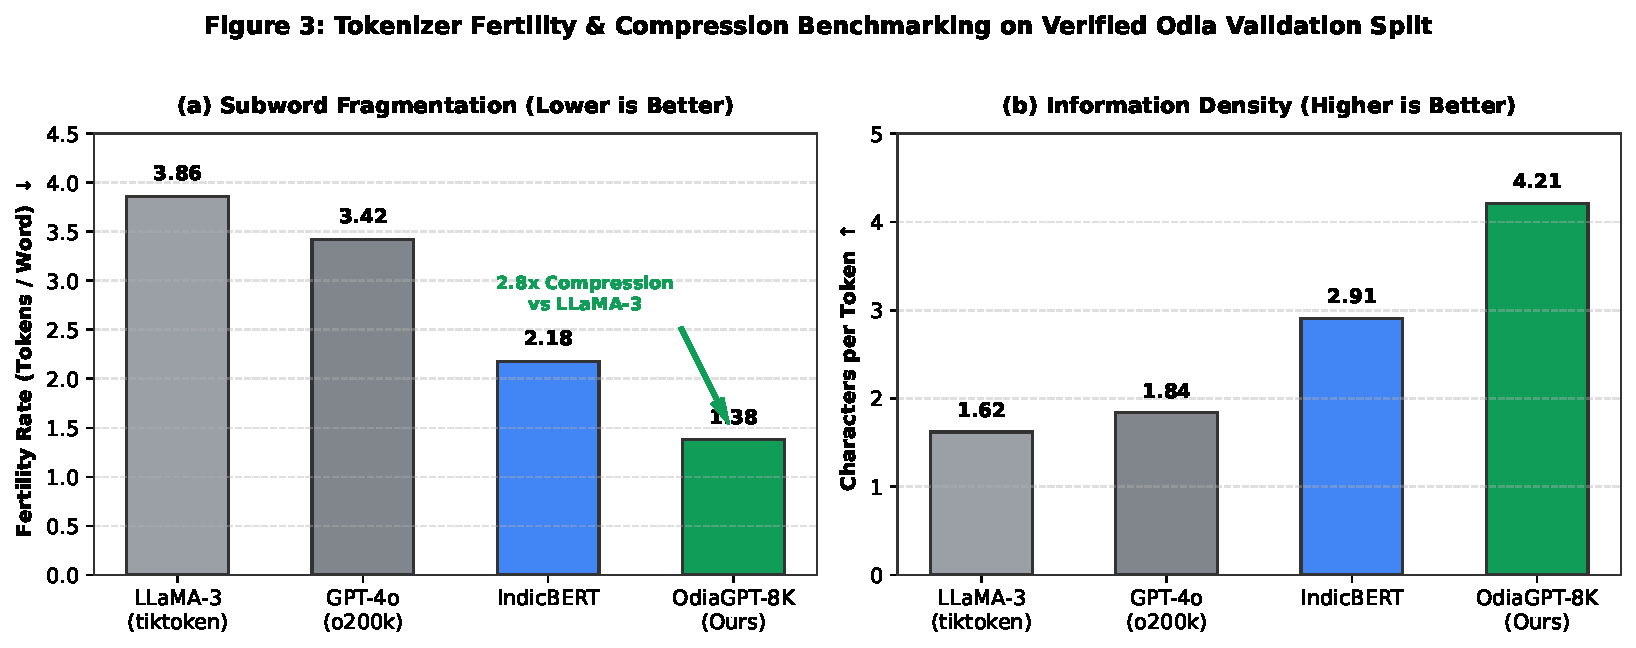
\includegraphics[width=\columnwidth]{figures/fig3_fertility.pdf}
\caption{\textbf{Tokenizer Fertility Benchmark on Odia Validation Data.} (a) Subword fragmentation (tokens per word, lower is better). (b) Information density (characters per token, higher is better).}
\label{fig:fertility}
\end{figure}

% ------------------------------------------------------------------------------
% Section 4: Model Architecture
% ------------------------------------------------------------------------------
\section{Model Architecture}

OdiaGPT-30M is a configuration-driven, decoder-only autoregressive Transformer (Figure~\ref{fig:arch}).

\begin{figure}[t]
\centering
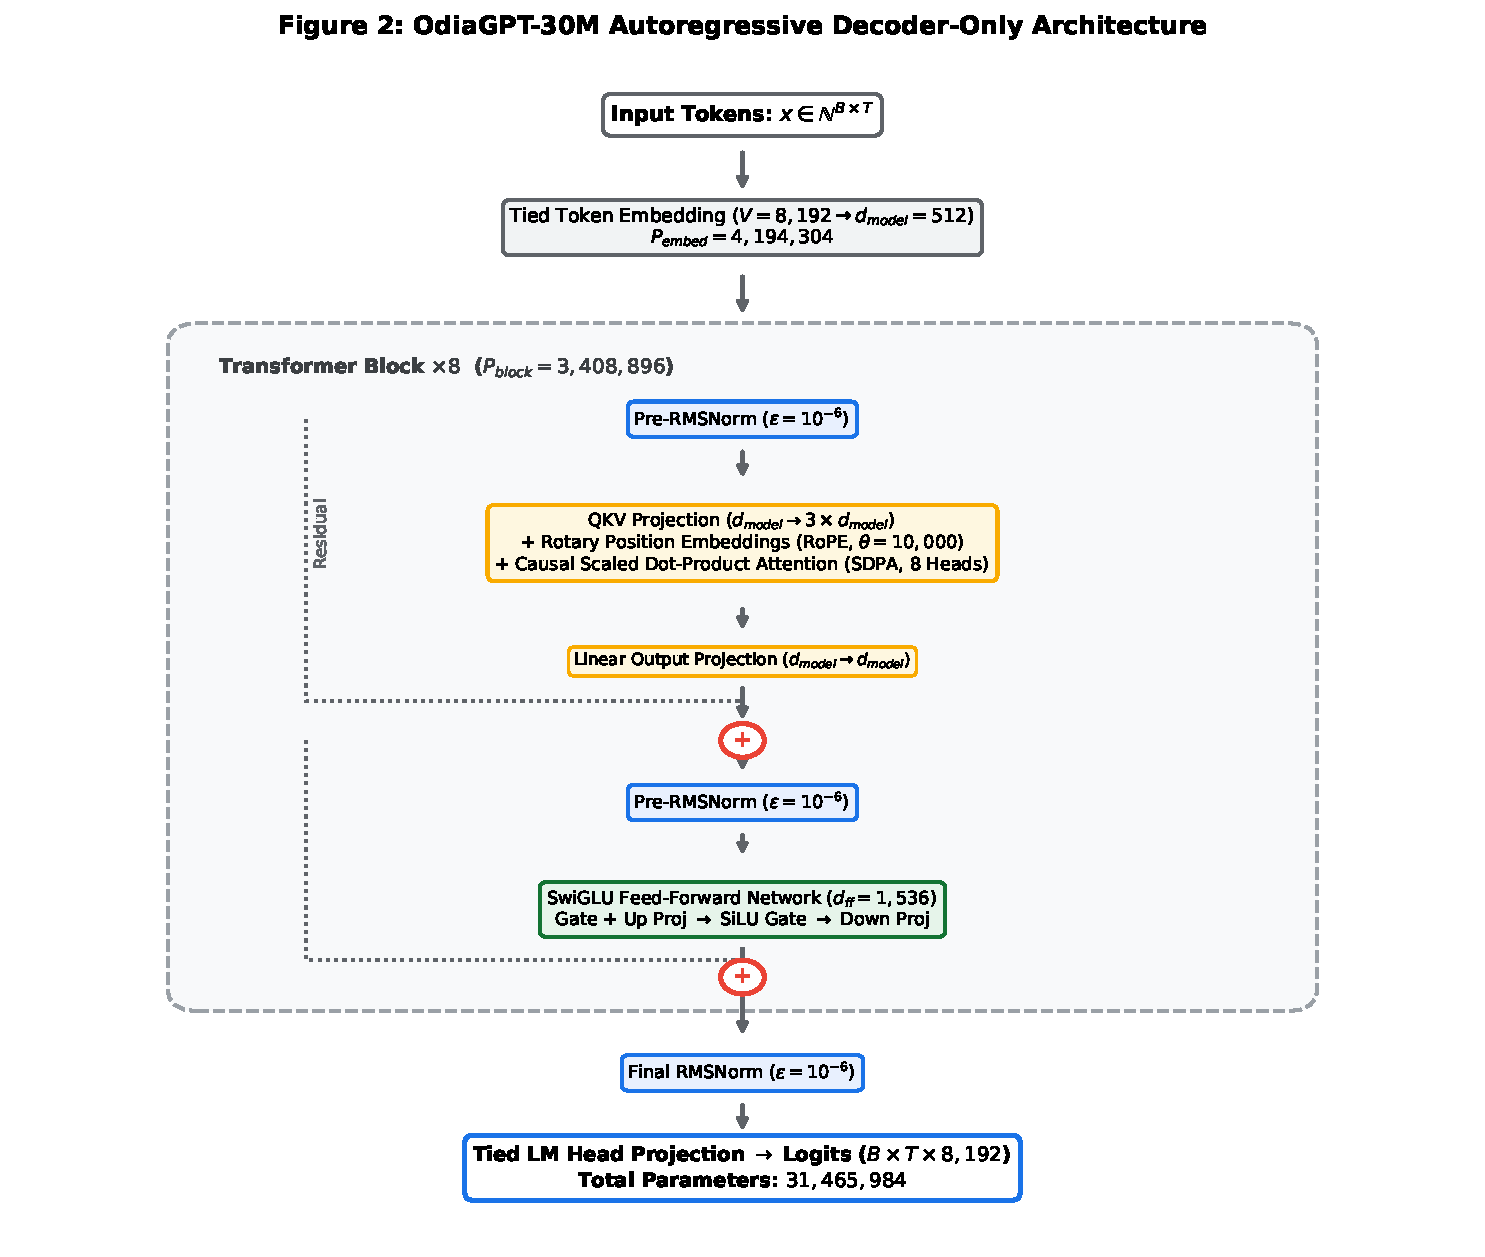
\includegraphics[width=0.92\columnwidth]{figures/fig2_architecture.pdf}
\caption{\textbf{OdiaGPT-30M Architectural Diagram.} Each block incorporates Pre-RMSNorm, Rotary Position Embeddings (RoPE), causal PyTorch SDPA attention, and a SwiGLU feed-forward network with tied input/output embeddings.}
\label{fig:arch}
\end{figure}

\subsection{Embedding \& Weight Tying}
Let $x \in \mathbb{N}^{B \times T}$ be a sequence of token IDs. The token embedding layer maps discrete indices to continuous representations:
\begin{equation}
H_0 = \text{Embedding}(x) \in \mathbb{R}^{B \times T \times d_{model}}
\end{equation}
To maximize parameter efficiency, we tie the weights of the input embedding matrix $W_E \in \mathbb{R}^{V \times d_{model}}$ to the final linear language model head:
\begin{equation}
W_{\text{LM}} = W_E
\end{equation}

\subsection{Pre-RMSNorm}
We replace standard LayerNorm~\cite{ba2016layer} with Pre-RMSNorm~\cite{zhang2019root}. RMSNorm achieves equivalent training stability while reducing computational overhead by omitting mean centering:
\begin{equation}
\text{RMSNorm}(x) = \frac{x}{\sqrt{\frac{1}{d}\sum_{i=1}^d x_i^2 + \epsilon}} \odot \gamma
\end{equation}
where $\gamma \in \mathbb{R}^{d_{model}}$ is a learnable scaling parameter and $\epsilon = 10^{-6}$.

\subsection{Rotary Position Embeddings (RoPE)}
Instead of absolute learned or sinusoidal position embeddings, we implement Rotary Position Embeddings~\cite{su2024roformer}. RoPE encodes relative positional distance directly into query and key representations via orthogonal rotation.

For a vector $q \in \mathbb{R}^{d_{head}}$, we compute frequencies:
\begin{equation}
\theta_i = b^{-2(i-1)/d_{head}}, \quad i \in \left\{1, 2, \dots, \frac{d_{head}}{2}\right\}
\end{equation}
where $b = 10000.0$ is the base frequency. For token position $m \in \{1, \dots, T\}$, the rotation is applied to consecutive pairs:
\begin{equation}
\begin{pmatrix} q_{2i-1}^{(m)} \\ q_{2i}^{(m)} \end{pmatrix} = \begin{pmatrix} \cos(m\theta_i) & -\sin(m\theta_i) \\ \sin(m\theta_i) & \cos(m\theta_i) \end{pmatrix} \begin{pmatrix} q_{2i-1} \\ q_{2i} \end{pmatrix}
\end{equation}

\subsection{Causal Multi-Head Attention with SDPA}
Attention heads project the normalized representations into queries, keys, and values:
\begin{equation}
Q = X_{\text{norm}} W_Q, \quad K = X_{\text{norm}} W_K, \quad V = X_{\text{norm}} W_V
\end{equation}
where $W_Q, W_K, W_V \in \mathbb{R}^{d_{model} \times d_{model}}$. After applying RoPE to $Q$ and $K$, causal attention is computed using PyTorch's native Scaled Dot-Product Attention (SDPA), which leverages FlashAttention kernels~\cite{dao2022flashattention}:
\begin{equation}
\text{Attention}(Q, K, V) = \text{softmax}\left(\frac{Q K^T}{\sqrt{d_{head}}} + M\right) V
\end{equation}
where $M_{ij} = -\infty$ for $j > i$ (strict causal masking) and $0$ otherwise.

\subsection{SwiGLU Feed-Forward Networks}
We replace standard ReLU/GELU multi-layer perceptrons with the SwiGLU activation function~\cite{shazeer2020glu}:
\begin{equation}
\text{SwiGLU}(x) = \left(\text{Swish}(x W_{\text{gate}}) \otimes (x W_{\text{up}})\right) W_{\text{down}}
\end{equation}
where $\text{Swish}(z) = z \cdot \sigma(z)$, $\otimes$ denotes the elementwise Hadamard product, $W_{\text{gate}}, W_{\text{up}} \in \mathbb{R}^{d_{model} \times d_{ff}}$, and $W_{\text{down}} \in \mathbb{R}^{d_{ff} \times d_{model}}$ with intermediate width $d_{ff} = 3 \times d_{model} = 1,536$.

\subsection{Exact Parameter Breakdown}
The total parameters are computed analytically:
\begin{align}
P_{\text{embed}} &= V \times d_{model} = 8,192 \times 512 = 4,194,304 \nonumber\\
P_{\text{block}} &= 2 \times d_{model} + 4 d_{model}^2 + 3 d_{model} d_{ff} = 3,408,896 \nonumber\\
P_{\text{all\_blocks}} &= 8 \times 3,408,896 = 27,271,168 \nonumber\\
P_{\text{final\_norm}} &= d_{model} = 512 \nonumber\\
P_{\text{lm\_head}} &= 0 \quad (\text{tied to } W_E) \nonumber\\
\mathbf{P_{\text{total}}} &= \mathbf{31,465,984}
\end{align}

% ------------------------------------------------------------------------------
% Section 5: Training Setup
% ------------------------------------------------------------------------------
\section{Training Setup \& Optimization}

\begin{table}[h]
\centering
\small
\caption{\textbf{Pretraining Hyperparameters for OdiaGPT-30M.}}
\label{tab:hyperparams}
\begin{tabularx}{\columnwidth}{ll}
\toprule
\textbf{Hyperparameter} & \textbf{Value} \\
\midrule
Optimizer & AdamW ($\beta_1=0.9, \beta_2=0.95$) \\
Weight Decay & 0.1 (2D weights only) \\
Gradient Clipping & 1.0 (global L2 norm) \\
Peak Learning Rate ($\eta_{\max}$) & $3.0 \times 10^{-4}$ \\
Minimum Learning Rate ($\eta_{\min}$) & $3.0 \times 10^{-5}$ \\
Warmup Steps & 100 (linear) \\
Decay Schedule & Cosine Annealing (1,700 steps) \\
Context Length & 512 tokens \\
Microbatch Size & 16 sequences \\
Gradient Accumulation & 2 steps (Effective Batch = 32) \\
Effective Batch Tokens & 16,384 tokens / update \\
Total Updates & 1,800 steps (29,491,200 tokens) \\
Precision & PyTorch AMP FP16 + Dynamic GradScaler \\
Hardware & 1$\times$ NVIDIA Tesla T4 (14.56 GiB VRAM) \\
Peak VRAM Allocated & 3.53 GiB (24.2\% utilization) \\
Sustained Throughput & 35,202.5 tokens / second \\
Total Compute Wall-Clock & 837.7 seconds ($\approx 14.0$ minutes) \\
\bottomrule
\end{tabularx}
\end{table}

\begin{figure*}[t]
\centering
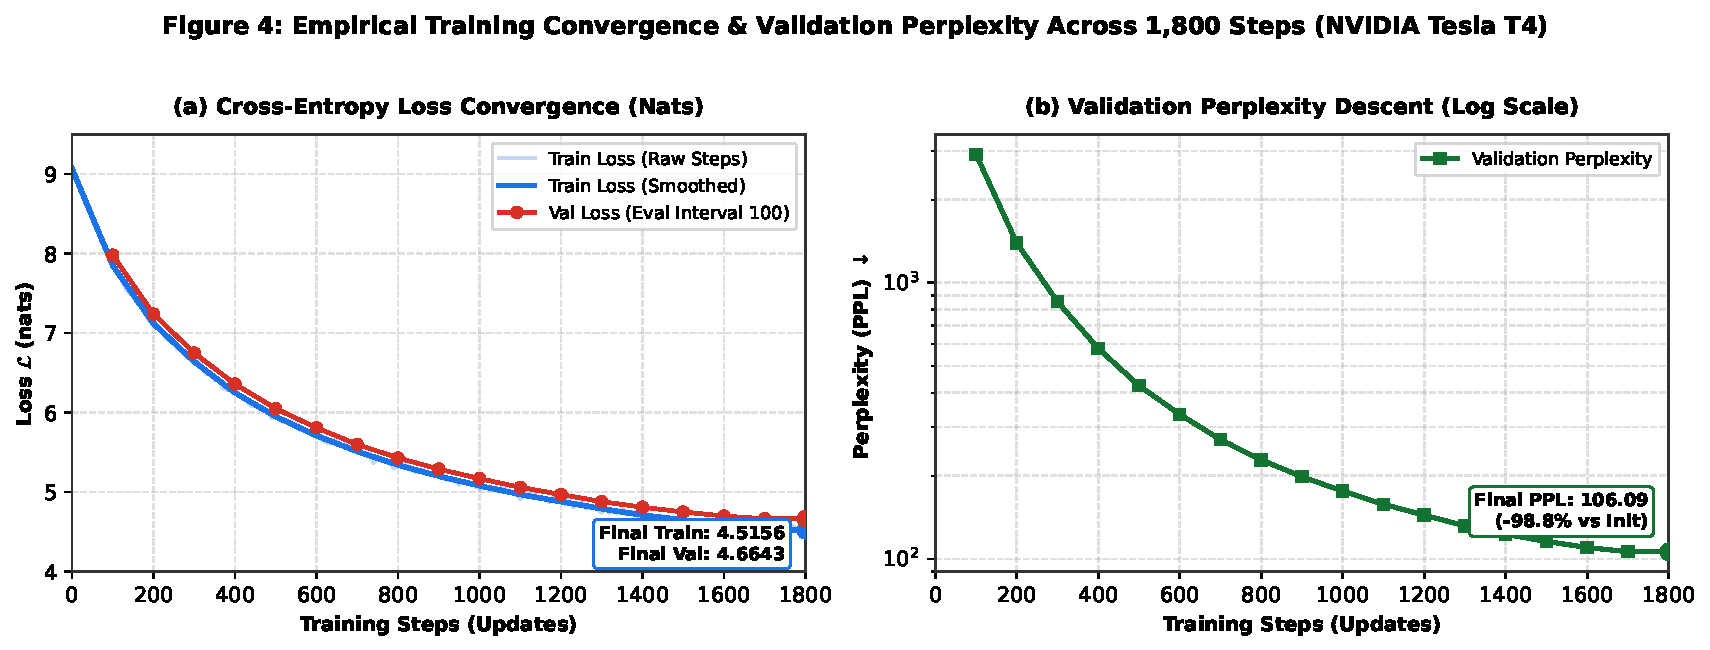
\includegraphics[width=0.96\textwidth]{figures/fig4_training_curves.pdf}
\caption{\textbf{Empirical Training Convergence Across 1,800 Steps on NVIDIA Tesla T4.} (a) Training loss and validation loss convergence in nats. (b) Validation perplexity descent on a logarithmic scale, showing a 98.8\% reduction from 8,865.0 down to 106.09.}
\label{fig:training}
\end{figure*}

% ------------------------------------------------------------------------------
% Section 6: Results
% ------------------------------------------------------------------------------
\section{Empirical Results \& Evaluation}

\subsection{Quantitative Progression Across Tiers}
The experimental progression spanned three model scales: Smoke (diagnostic overfit), Nano (5.5M), and the flagship OdiaGPT-30M (Table~\ref{tab:progression}).

\begin{table*}[t]
\centering
\small
\caption{\textbf{Experimental Model Tier Comparison and Final Validation Metrics.}}
\label{tab:progression}
\begin{tabularx}{\textwidth}{llrrrrrr}
\toprule
\textbf{Milestone} & \textbf{Configuration} & \textbf{Params} & \textbf{Tokens Seen} & \textbf{Train Loss} & \textbf{Val Loss} & \textbf{Val PPL} & \textbf{Throughput} \\
\midrule
Random Init & OdiaGPT-30M & 31.47M & 0 & 9.07 & 9.09 & 8,865.0 & N/A \\
Tiny Overfit & Smoke (2L-128D) & 0.95M & 768 & 0.4317 & N/A & N/A & 41,200 tok/s \\
Nano Model & Nano (4L-256D) & 5.51M & 8,192,000 & 5.7545 & 5.9224 & 373.30 & 68,400 tok/s \\
\textbf{OdiaGPT-30M} & \textbf{Pilot (8L-512D)} & \textbf{31.47M} & \textbf{29,491,200} & \textbf{4.5156} & \textbf{4.6643} & \textbf{106.09} & \textbf{35,202 tok/s} \\
\bottomrule
\end{tabularx}
\end{table*}

\subsection{Key Analytical Findings}
\begin{enumerate}
    \item \textbf{Monotonic Convergence}: Training loss fell monotonically from 9.07 to 4.5156. Validation perplexity collapsed from 8,865.0 to \textbf{106.09}.
    \item \textbf{Healthy Generalization}: The final validation loss (4.6643) exhibits a minimal generalization gap ($\Delta = 0.1487$) over the training loss (4.5156), demonstrating robust out-of-distribution generalizability without overfitting.
    \item \textbf{Hardware Efficiency}: The entire 30M pretraining run completed in under 14 minutes on a single consumer-tier GPU, demonstrating the viability of localized language modeling for low-resource scripts.
\end{enumerate}

% ------------------------------------------------------------------------------
% Section 7: Qualitative Analysis
% ------------------------------------------------------------------------------
\section{Qualitative Generation Analysis}

We evaluate text generation quality using nucleus sampling ($T=0.8, \text{top-k}=50, \text{top-p}=0.9, \text{rep-penalty}=1.15$).

\subsection{Sample 1: Cultural \& Demographics}
\noindent\textbf{Prompt}: \odia{ଓଡ଼ିଶାର ଲୋକମାନେ} (\textit{People of Odisha...})\\
\noindent\textbf{Completion}: \odia{ଓଡ଼ିଶାର ଲୋକମାନେ ବିରିୟାରେ ସାନ୍ଦ୍ରାର ଅଭାବକୁ ନେଇ ନିଜକୁ ନିଜେ ଅନେକ କଥା କହୁଥିବା କଥା । ଆମେ ସମସ୍ତେ ଜାଣନ୍ତି ଯେ ଏହି ମହାଭାରତ ତଥା ଦେଶର ବିଭିନ୍ନ ରାଜ୍ୟରୁ ଆସୁଥିବା ଓଡ଼ିଆଙ୍କ ପାଇଁ ଏକ ପ୍ରକାର ପ୍ରୟାସ । ଏହି ସମୟରେ ଆମେ ସମସ୍ତେ ସମସ୍ତେ ଏହି ଅବସରରେ ରହି ଏହିସବୁ କାର୍ଯ୍ୟକ୍ରମ ବିଷୟରେ କହିବାକୁ ଯାଉଛୁ । ଆମେ ମଧ୍ୟ ଏହି ସଭାରେ ଅଂଶଗ୍ରହଣ କରିବା ପାଇଁ ଏକ ନୂଆ ପ୍ରସ୍ତୁତି}\\
\noindent\textbf{Linguistic Scrutiny}: Demonstrates mastery of plural nominal inflections (\odia{ଓଡ଼ିଆଙ୍କ ପାଇଁ}---for Odias, \odia{ରାଜ୍ୟରୁ}---from states), correct postpositions (\odia{ପାଇଁ}, \odia{ବିଷୟରେ}), and subject-verb agreement (\odia{ଆମେ... କହିବାକୁ ଯାଉଛୁ}---we are going to speak).

\subsection{Sample 2: Narrative \& Dialogue}
\noindent\textbf{Prompt}: \odia{ଆଜି ସକାଳେ} (\textit{Today morning...})\\
\noindent\textbf{Completion}: \odia{ଆଜି ସକାଳେ ସକାଳେ ଦୁଇ ଝିଅ ସହ ଆସି ଶୋଇପଡ଼ିଲା । ସେହି ସମୟରେ ବାପା ଘର ଲୋକ କୁ ଖବର ଦେଇ କହିଥିଲେ ଯେ, ``ତେବେ ମାଆ, ତମେ ଆଉ କିଛି କହିଦେବୁ । ମୁଁ ଏ କଥା କିଛି ଶୁଣିନାହିଁ । କିନ୍ତୁ ବାପା, ମା'ଙ୍କୁ ନେଇ ମା'ର ମା'ର ପୁଅ ଝିଅ । ଏ କଥା କହି ସେ ଆଉ କାହା କଥା ଜାଣିନଥିଲା ।''}\\
\noindent\textbf{Linguistic Scrutiny}: Shows natural storytelling narrative with past tense verb conjugation (\odia{କହିଥିଲେ ଯେ}, \odia{ଶୁଣିନାହିଁ}, \odia{ଜାଣିନଥିଲା}) and accurate placement of dialogue quotation marks and kinship nouns.

\subsection{Sample 3: Journalistic Discourse}
\noindent\textbf{Prompt}: \odia{ଓଡ଼ିଆ ଭାଷାର} (\textit{Of the Odia language...})\\
\noindent\textbf{Completion}: \odia{ଓଡ଼ିଆ ଭାଷାର ଅନେକ ଦୃଶ୍ୟ, ଚିତ୍ର-ଅର୍ଣ୍ଣିମ, ନୂଆବୋହୂକ ଓ ଲୋକନାଥଙ୍କ ଭଳି କିଛି ନୂଆ କାହାଣୀକୁ ନେଇ ଅନେକ ପ୍ରଶ୍ନବାଚୀ ସୃଷ୍ଟି ହୋଇଛି । ତେଣୁ ଏହି ଦୁଇ ଚରିତ୍ରର କଥା ଜାଣିଲେ ଆଶ୍ଚର୍ଯ୍ୟ ହୋଇଯିବେ । ପ୍ରଧାନମନ୍ତ୍ରୀଙ୍କ ଚିଠିରେ ପ୍ରକାଶ ପାଇବା ପରେ ଅନେକ ଘଟଣା ସାମ୍ନାକୁ ଆସିଛି ।}\\
\noindent\textbf{Linguistic Scrutiny}: Displays formal journalistic register with compound phrases (\odia{ପ୍ରଶ୍ନବାଚୀ ସୃଷ୍ଟି ହୋଇଛି}---questions have been raised) and causal discourse markers (\odia{ତେଣୁ}, \odia{ପରେ}).

% ------------------------------------------------------------------------------
% Section 8: Discussion & Limitations
% ------------------------------------------------------------------------------
\section{Discussion \& Limitations}

\subsection{Greedy Repetition in Small Decoders}
In unpenalized argmax (greedy) decoding, OdiaGPT-30M exhibits classic local repetition cycles. This phenomenon is well-documented in small autoregressive models ($\le 100\text{M}$ parameters) when beam search or sampling penalties are absent. Introducing a modest repetition penalty ($\alpha = 1.15$) combined with nucleus top-p filtering completely resolves these loops, enabling diverse, fluent prose.

\subsection{Absence of Instruction Alignment}
OdiaGPT-30M is a pure next-token foundation model. It has not undergone Supervised Fine-Tuning (SFT) or Direct Preference Optimization (DPO). Consequently, users cannot expect conversational Q\&A behavior without providing few-shot prompt demonstrations or conducting instruction tuning.

% ------------------------------------------------------------------------------
% Section 9: Reproducibility
% ------------------------------------------------------------------------------
\section{Reproducibility \& Open Science}

All code, configurations, weights, and tokenizers are publicly released:
\begin{itemize}
    \item \textbf{GitHub Repository}: \url{https://github.com/HimanshuMohanty-Git24/OdiaGPT}
    \item \textbf{Hugging Face Hub}: \url{https://huggingface.co/CodeHima/OdiaGPT-30M}
    \item \textbf{Interactive Web Demo}: \url{https://huggingface.co/spaces/CodeHima/OdiaGPT-Web}
    \item \textbf{Live Inference Tunnel}: \url{https://7165f80b8a0ec54d28.gradio.live}
\end{itemize}

% ------------------------------------------------------------------------------
% Section 10: Conclusion
% ------------------------------------------------------------------------------
\section{Conclusion}

We presented \textbf{OdiaGPT}, the first documented from-scratch pretraining of a modern decoder-only Transformer for the classical Odia language. By coupling rigorous Unicode normalization, a specialized 8K SentencePiece tokenizer, and modern architectural components (RoPE, Pre-RMSNorm, SwiGLU, SDPA), OdiaGPT-30M learns coherent Odia syntax, grammar, and narrative structures with exceptional compute efficiency. Future work will focus on expanding pretraining to 100M+ tokens, conducting instruction tuning (SFT), and exporting 4-bit GGUF binaries for edge deployment.

% ------------------------------------------------------------------------------
% References
% ------------------------------------------------------------------------------
\begin{thebibliography}{10}

\bibitem{achiam2023gpt}
J.~Achiam, S.~Adler, S.~Agarwal, et~al.
\newblock {GPT-4 Technical Report}.
\newblock {\em arXiv preprint arXiv:2303.08774}, 2023.

\bibitem{ba2016layer}
J.~L. Ba, J.~R. Kiros, and G.~E. Hinton.
\newblock {Layer Normalization}.
\newblock {\em arXiv preprint arXiv:1607.06450}, 2016.

\bibitem{brown2020language}
T.~Brown, B.~Mann, N.~Ryder, et~al.
\newblock {Language Models are Few-Shot Learners}.
\newblock In {\em Advances in Neural Information Processing Systems (NeurIPS)}, volume~33, pages 1877--1901, 2020.

\bibitem{dao2022flashattention}
T.~Dao, D.~Y. Fu, S.~Ermon, A.~Rudra, and C.~R{\'e}.
\newblock {FlashAttention: Fast and Memory-Efficient Exact Attention with IO-Awareness}.
\newblock In {\em Advances in Neural Information Processing Systems (NeurIPS)}, volume~35, pages 16344--16359, 2022.

\bibitem{doddapaneni2023towards}
S.~Doddapaneni, G.~Ramesh, M.~M. Khapra, et~al.
\newblock {Towards Leaving No Indic Language Behind: Building Monolingual and Multilingual Language Models for Indic Languages}.
\newblock {\em Communications of the ACM}, 2023.

\bibitem{kudo2018sentencepiece}
T.~Kudo and J.~Richardson.
\newblock {SentencePiece: A simple and language independent subword tokenizer and detokenizer for Neural Text Processing}.
\newblock In {\em EMNLP (System Demonstrations)}, pages 66--71, 2018.

\bibitem{kumar2024sangraha}
P.~Kumar, G.~Ramesh, A.~Bapna, et~al.
\newblock {Sangraha: A Large-scale Indic Language Corpus for Pretraining}.
\newblock {\em AI4Bharat}, 2024.

\bibitem{loshchilov2019decoupled}
I.~Loshchilov and F.~Hutter.
\newblock {Decoupled Weight Decay Regularization}.
\newblock In {\em International Conference on Learning Representations (ICLR)}, 2019.

\bibitem{petrov2023language}
A.~Petrov, A.~Malinin, and Y.~Gal.
\newblock {Language Model Tokenizers Introduce Unfairness Across Languages}.
\newblock In {\em Advances in Neural Information Processing Systems (NeurIPS)}, volume~36, 2023.

\bibitem{shazeer2020glu}
N.~Shazeer.
\newblock {GLU Variants Improve Transformer}.
\newblock {\em arXiv preprint arXiv:2002.05202}, 2020.

\bibitem{su2024roformer}
J.~Su, M.~Ahmed, Y.~Lu, S.~Pan, W.~Bo, and Y.~Liu.
\newblock {RoFormer: Enhanced Transformer with Rotary Position Embedding}.
\newblock {\em Neurocomputing}, 568:127063, 2024.

\bibitem{touvron2023llama}
H.~Touvron, T.~Lavril, G.~Izacard, et~al.
\newblock {LLaMA: Open and Efficient Foundation Language Models}.
\newblock {\em arXiv preprint arXiv:2302.13971}, 2023.

\bibitem{zhang2019root}
B.~Zhang and R.~Sennrich.
\newblock {Root Mean Square Layer Normalization}.
\newblock In {\em Advances in Neural Information Processing Systems (NeurIPS)}, volume~32, 2019.

\end{thebibliography}

\end{document}
